\documentclass[journal]{vgtc}                % final (journal style)
%\documentclass[review,journal]{vgtc}         % review (journal style)
%\documentclass[widereview]{vgtc}             % wide-spaced review
%\documentclass[preprint,journal]{vgtc}       % preprint (journal style)

%% Uncomment one of the lines above depending on where your paper is
%% in the conference process. ``review'' and ``widereview'' are for review
%% submission, ``preprint'' is for pre-publication, and the final version
%% doesn't use a specific qualifier.

%% Please use one of the ``review'' options in combination with the
%% assigned online id (see below) ONLY if your paper uses a double blind
%% review process. Some conferences, like IEEE Vis and InfoVis, have NOT
%% in the past.

%% Please note that the use of figures other than the optional teaser is not permitted on the first page
%% of the journal version.  Figures should begin on the second page and be
%% in CMYK or Grey scale format, otherwise, colour shifting may occur
%% during the printing process.  Papers submitted with figures other than the optional teaser on the
%% first page will be refused. Also, the teaser figure should only have the
%% width of the abstract as the template enforces it.

%% These few lines make a distinction between latex and pdflatex calls and they
%% bring in essential packages for graphics and font handling.
%% Note that due to the \DeclareGraphicsExtensions{} call it is no longer necessary
%% to provide the the path and extension of a graphics file:
%% 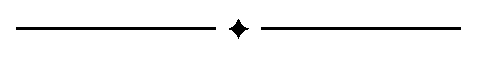
\includegraphics{diamondrule} is completely sufficient.
%%
\ifpdf%                                % if we use pdflatex
  \pdfoutput=1\relax                   % create PDFs from pdfLaTeX
  \pdfcompresslevel=9                  % PDF Compression
  \pdfoptionpdfminorversion=7         % create PDF 1.7
  \ExecuteOptions{pdftex}
  \usepackage{graphicx}  
  \graphicspath{ {pictures/} }              % allow us to embed graphics files
  \DeclareGraphicsExtensions{.pdf,.png,.jpg,.jpeg} % for pdflatex we expect .pdf, .png, or .jpg files
\else%                                 % else we use pure latex
  \ExecuteOptions{dvips}
  \usepackage{graphicx}                % allow us to embed graphics files
  \DeclareGraphicsExtensions{.eps}     % for pure latex we expect eps files
\fi%

%% it is recomended to use ``\autoref{sec:bla}'' instead of ``Fig.~\ref{sec:bla}''
\graphicspath{{figures/}{pictures/}{images/}{./}} % where to search for the images

\usepackage{microtype}                 % use micro-typography (slightly more compact, better to read)
\PassOptionsToPackage{warn}{textcomp}  % to address font issues with \textrightarrow
\usepackage{textcomp}                  % use better special symbols
\usepackage{mathptmx}                  % use matching math font
\usepackage{times}                     % we use Times as the main font
\renewcommand*\ttdefault{txtt}         % a nicer typewriter font
\usepackage{cite}                      % needed to automatically sort the references
\usepackage{tabu}                      % only used for the table example
\usepackage{booktabs}                  % only used for the table example
\usepackage[section]{placeins}
\usepackage{float}
\usepackage{hyperref}
\usepackage[all]{hypcap}
\usepackage{enumitem} 
\hypersetup{
    colorlinks = true,
    citecolor = {black},
    urlcolor = {red}
}

%% We encourage the use of mathptmx for consistent usage of times font
%% throughout the proceedings. However, if you encounter conflicts
%% with other math-related packages, you may want to disable it.

%% In preprint mode you may define your own headline.
%\preprinttext{To appear in IEEE Transactions on Visualization and Computer Graphics.}

%% If you are submitting a paper to a conference for review with a double
%% blind reviewing process, please replace the value ``0'' below with your
%% OnlineID. Otherwise, you may safely leave it at ``0''.
\onlineid{0}

%% declare the category of your paper, only shown in review mode
\vgtccategory{Research}
%% please declare the paper type of your paper to help reviewers, only shown in review mode
%% choices:
%% * algorithm/technique
%% * application/design study
%% * evaluation
%% * system
%% * theory/model

%% Paper title.
\title{An Evaluation of Poemage}

%% This is how authors are specified in the journal style

%% indicate IEEE Member or Student Member in form indicated below
\author{Daniel Schroeder, Will Sims, and Bungo Takahashi}
\authorfooter{
%% insert punctuation at end of each item
\item
 Daniel Schroeder is a computer science student at Oregon State University. E-mail: schrodan@oregonstate.edu.
\item
 BUNGO Takahashi is a computer science student at Oregon State University. E-mail: takahasb@oregonstate.edu.
\item
 Will Sims is a computer science student at Oregon State University.\break E-mail: simsw@oregonstate.edu.
}

%other entries to be set up for journal
%\shortauthortitle{Biv \MakeLowercase{\textit{et al.}}: Crimes on Oregon College Campuses}
%\shortauthortitle{Firstauthor \MakeLowercase{\textit{et al.}}: Paper Title}

%% Abstract section.
\abstract{This paper is a visualization evaluation of the program Poemage, created by Nina McCurdy, Julie Lein, Katharine Coles, and Miriah Meyer from the University of Utah. We will evaluate the effectiveness of this visualization as well as suggest future implementations that could enhance the application. %
} % end of abstract

%% Keywords that describe your work. Will show as 'Index Terms' in journal
%% please capitalize first letter and insert punctuation after last keyword
\keywords{Visualization in the humanities, design studies, text and document data, graph/network data, text highlighting, evaluation and usability, poemage}

%% ACM Computing Classification System (CCS). 
%% See <http://www.acm.org/class/1998/> for details.
%% The ``\CCScat'' command takes four arguments.

\CCScatlist{ % not used in journal version
 \CCScat{K.6.1}{Management of Computing and Information Systems}%
{Project and People Management}{Life Cycle};
 \CCScat{K.7.m}{The Computing Profession}{Miscellaneous}{Ethics}
}

%% Uncomment below to include a teaser figure.
\teaser{
  \centering
  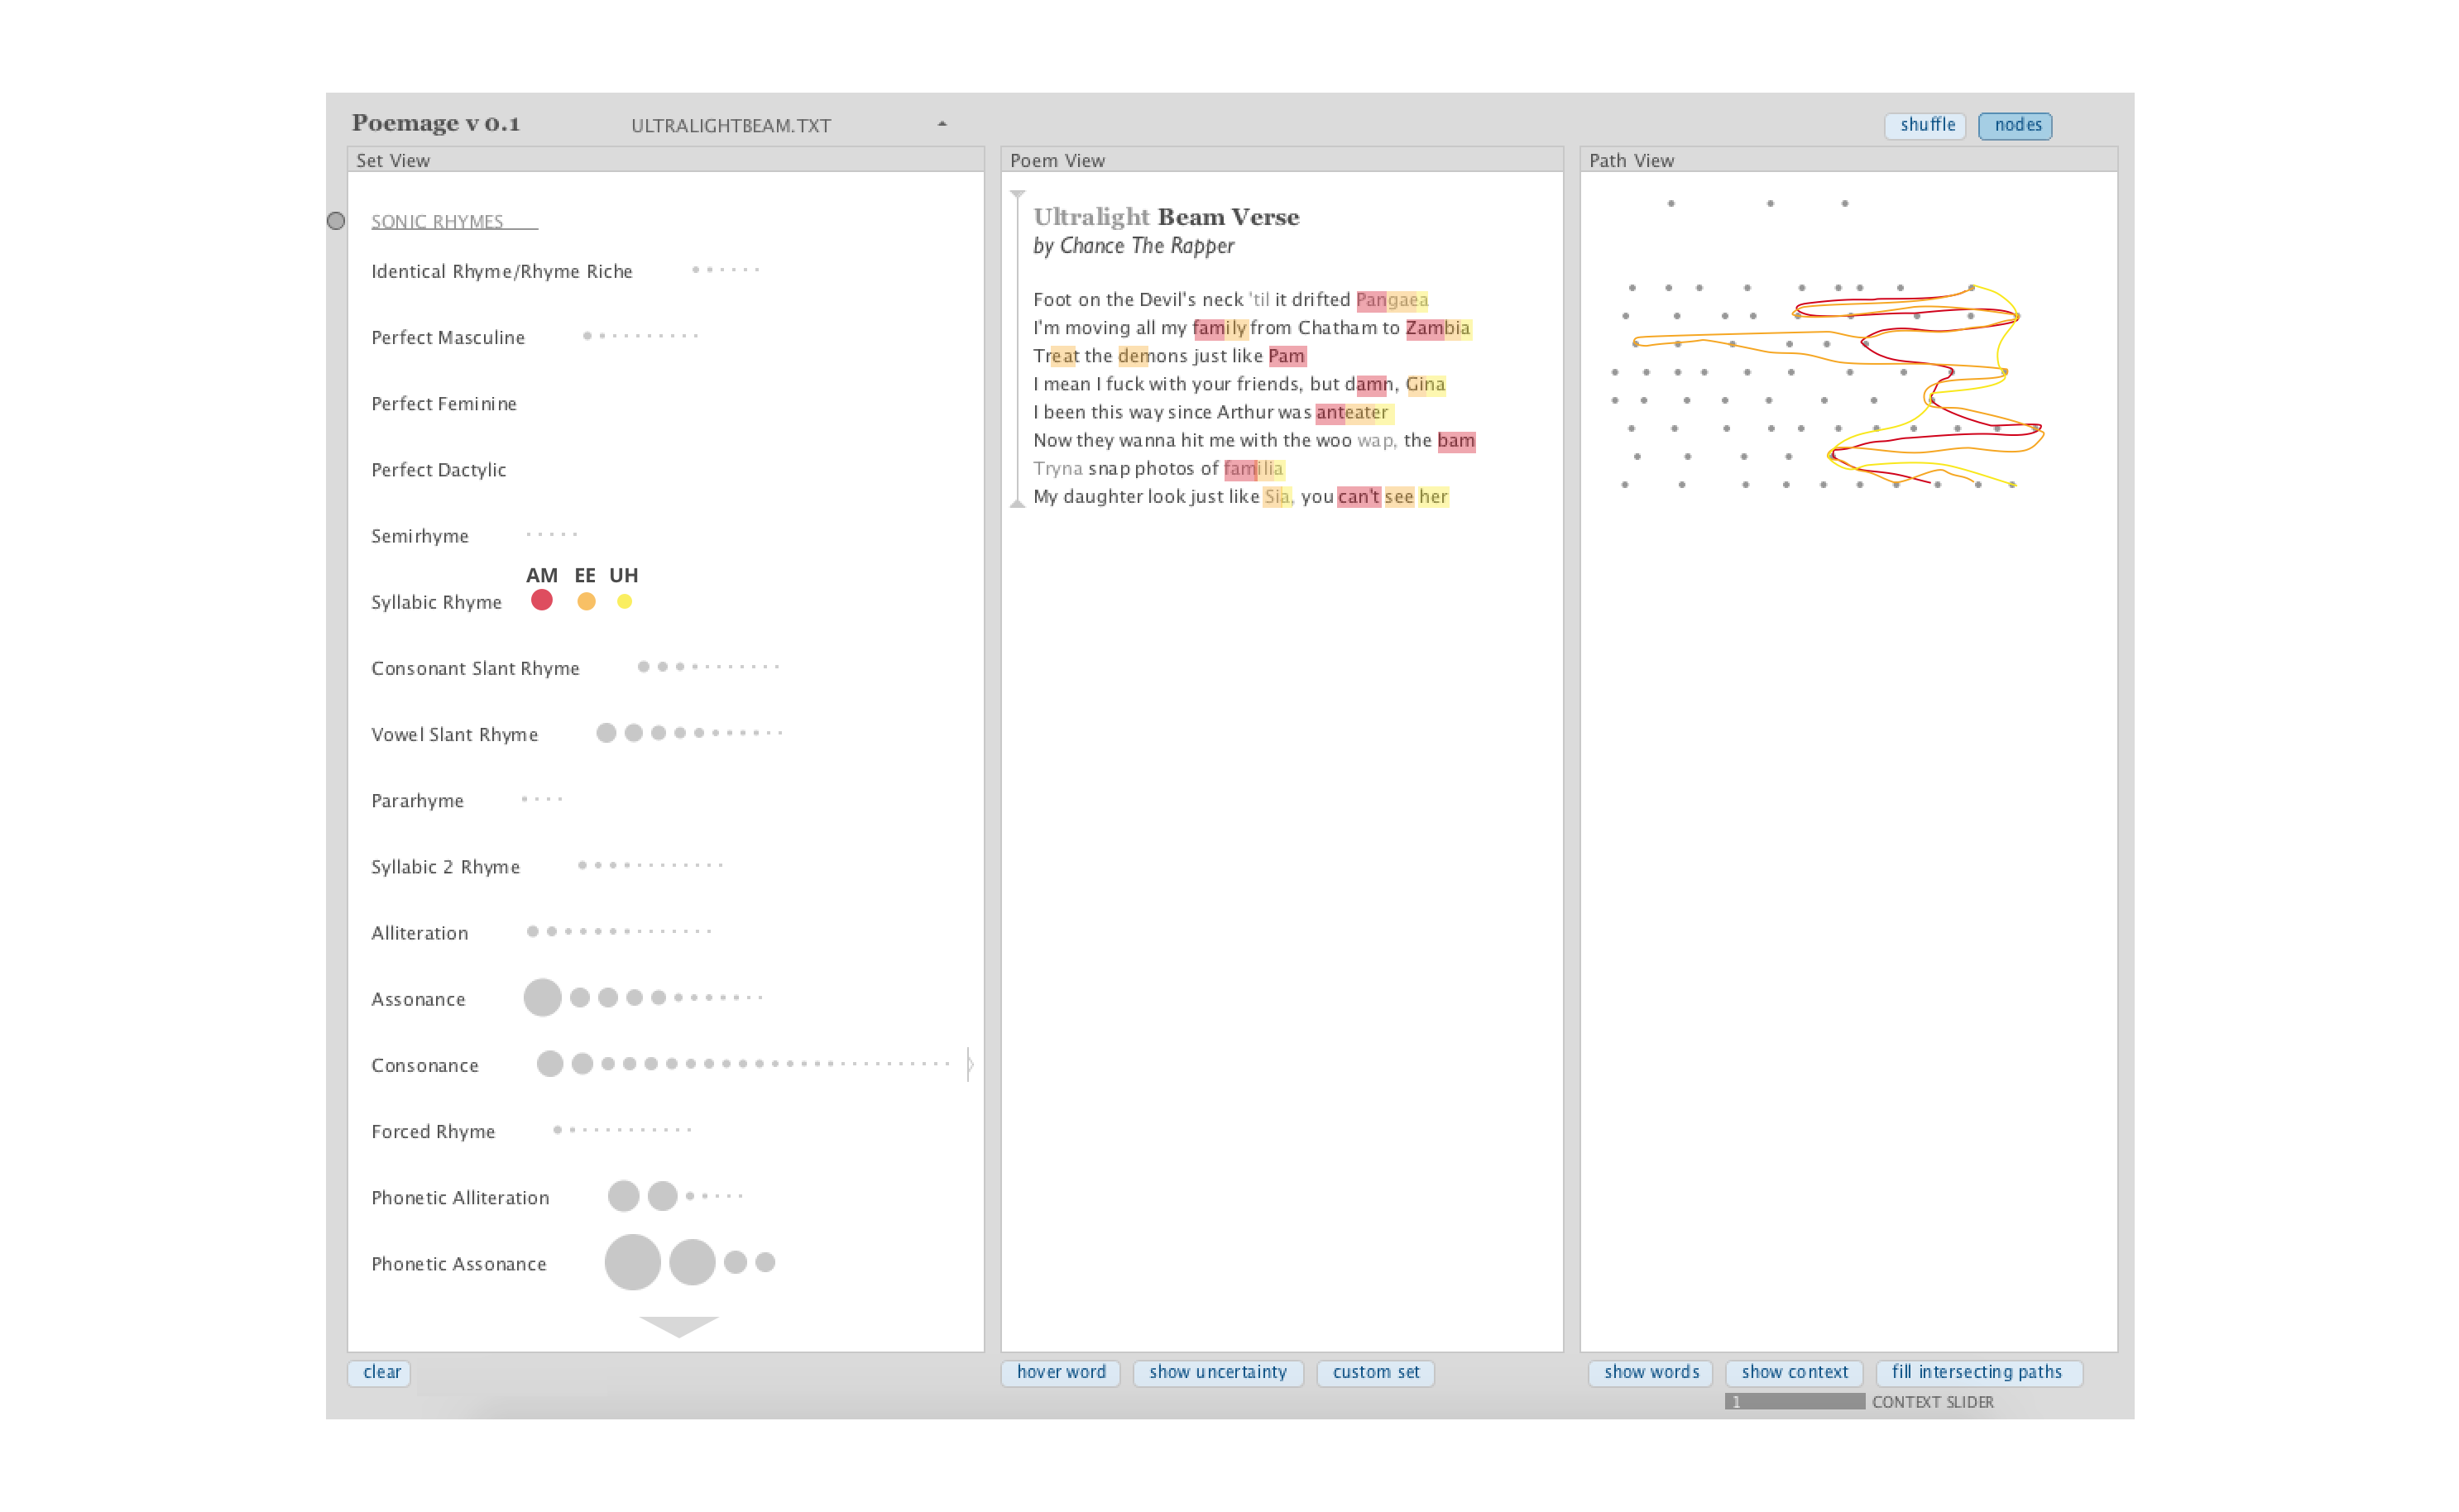
\includegraphics[width=\linewidth]{Redesign.png}
  \caption{This is our proposed redesign of the Poemage interface. Some notable differences are the use of text highlighting instead of ellipses, improved spacing between syllables within the set view, and an arrow to inform the user that ther is more information below sonic rhymes. The improvements were based off the results from our usability testing.}
	\label{fig:teaser}
}

%% Uncomment below to disable the manuscript note
\renewcommand{\manuscriptnotetxt}{}

%% Copyright space is enabled by default as required by guidelines.
%% It is disabled by the 'review' option or via the following command:
% \nocopyrightspace

\vgtcinsertpkg

%%%%%%%%%%%%%%%%%%%%%%%%%%%%%%%%%%%%%%%%%%%%%%%%%%%%%%%%%%%%%%%%
%%%%%%%%%%%%%%%%%%%%%% START OF THE PAPER %%%%%%%%%%%%%%%%%%%%%%
%%%%%%%%%%%%%%%%%%%%%%%%%%%%%%%%%%%%%%%%%%%%%%%%%%%%%%%%%%%%%%%%%

\begin{document}

%% The ``\maketitle'' command must be the first command after the
%% ``\begin{document}'' command. It prepares and prints the title block.

%% the only exception to this rule is the \firstsection command
\firstsection{Introduction}

\maketitle
\subsection{What is Poemage}
Poemage is a sonic topology visualization tool for poetry. The project was designed and created by a team of computer scientists and poets at the University of Utah. Poemage contains three types of data which are poem space, rhyme sets, and sonic topology. In Poemage, words have their own locations defined by the word’s position in a line and the line’s position in the poem space.  In addition to that, words belong to rhyme sets which are calculated by Poemage’s rhyming scheme, and there are 24 different kinds of rhyme types in the current version of Poemage. Then, sonic topology is calculated based on those sets of words classified in rhyme sets. Using those three attributes, Poemage visualizes sonic topology of poems and help users understand how words in a poem relate to one another.
\subsection{Problem}
 The problem behind the project was how the computer can contribute to close reading. In general, there are two types of reading: distant reading and close reading. In distant reading, {\it``It aims to generate an abstract view by shifting from observing textual content to visualizing global features of a single or of multiple text(s)''.} \cite{reading} On the contrary, in close reading, it includes analysis on individuals, events, and ideas, their development and interaction, used words and phrases, text structure and style, and argument patterns. \cite{reading} As we know, the computer can process a lot of data, and textual data is not an exception, which means it is good at distant reading. However, it has been a question if the computer can be used for close reading, because it requires analysis on a single text from a lot of viewpoints. Having said that, the project team from the University of Utah decided to create a tool that focuses on one of the aspects in close reading, which is sound, so that the computer can contribute to that type of reading.

\subsection{Purpose and Importance}
As explained earlier, close reading requires analysis on a single text from different points of view, and sound is one of them. Especially in poetry, the interaction of sonic devices between words is complex, which makes it hard for poets to analyze rhyme efficiently. The poemage project addresses this difficulty by visualizing sonic topology so as to generate productive meaning from poems in terms of sound, and it helps users understand relationships and interactions between words more effectively. This visualization is important because it is difficult for a human to capture all of the relationships between words and to analyze them by hand. In addition to that, the visualization gives users new perspectives which they had not realized. Therefore, it is beneficial to visualize sound topology thoroughly by utilizing the software.


\section{Related Work} \label{research}

Close reading through computational means is a very difficult problem to tackle due to its large problem set and complexity by nature. Most design decisions for computational close reading tend to focus on a specific area of interest within close reading, for example sound or rhyme. Nina McCurdy from The University of Utah wrote: ``Close reading covers a broad range of tasks, encompasses varying styles of analysis, allows many different points of entry, and accepts an extensive range of sometimes radically divergent interpretations'' when describing the complexity of text analysis \cite{poemage}.\\
\indent There have been numerous previous projects trying to tackle close reading via visualization and computation like E-Margin \cite{emargin}, Serendip \cite{serendip}, and Myopia \cite{myopia}. The Poemage team took a slightly different course during their development by focusing on sounds and creating a program that could ``automatically sonify a poem'' \cite{poemage}. All previous projects address the problem of close reading as an interpretation of text at the level of individual words in order to interpret and examine literary context. A large issue with addressing this problem is that it is usually done in an academic setting where someone is trying to ``teach'' the literature, and hand written evaluations tend to be messy and difficult to understand. These close reading visualization projects attempt to help visualize textual interpretations so that it can be taught and evaluated easily and effectively.\\
\indent We wanted to branch off from the Poemage style of using drawn ellipses to highlight words of interest and search for other methods of text highlighting that may increase the effectiveness of the visualization. We sought to highlight individual syllables or letters that applied to the filtered rhyme scheme or rhyme rule rather than circling the entire word. There has been extensive research on text highlighting techniques conducted by the information visualization community. A paper from IEEE Transactions on Visualization and Computer Graphics states that ``Text highlighting is important in any scenario where close reading (sequential word-by-word reading) is required and text annotations exist, that should be made accessible to the reader'' \cite{texthighlighting}. We wanted to explore the possibilities of using background coloring to target different parts of a single word to beautify the user interface as a whole and enhance the effectiveness of the Poemage program. By using different background colors used to target specific letters and syllables, the user will be able to clearly identify the sonic devices being targeted and be able to see where in the word it is present. The issue of where in the word the sonic device is located is not expressed through the use of drawn ellipses in the current version of Poemage, and users become overpowered with clutter and complexity when multiple filters are applied. 



\section{Method} \label{method}
In the methods section we discuss how we carried out the usability evaluation of Poemage and the evalution of Poemage with different languages.
\subsection{Method Overview}
Poemage is a tool that was created for close reading which is primarily used in education. 
We wanted to build on this application by making assessing how well it meets the needs of students and people that speak languages other than English. 
In order to accomplish this, we evaluated the effectiveness of Poemage while using different languages such as Spanish, and also conducted a usability evaluation to evaluate the ease of use of the application. 
\subsection{Usability Evaluation}
According to Nielsen, Usability is a quality attribute that assesses how easy user interfaces are to use. 
The word \textbf{usability} refers to methods for improving ease-of-use during the design process \cite{nielson}. 
Since it very likely Poemage will be used in an education setting, it is critical that students are able to understand how to use the application. 
Usability is especially important because Poemage is only useful when it is more efficient than analyzing a poem by hand. 
We conducted a cognitive walkthrough before creating our tasks for the usability evaluation so that we could find areas of interest that we would like to test with users.\break 
\indent The cognitive walkthrough showed that some of the problem areas may include the ambiguity of the modes section, overlapping text when selecting all parts of a sonic rhyme. 
It was also unclear whether or not there are more sonic rhymes below “Phonetic Assonance” in the set view, and it is difficult to see which syllables in a word are actually making the sound that rhymes with other words. 
We used these findings from the cognitive walkthrough to construct the tasks that users would perform for usability testing. 
\subsection{Tasks, Metrics, and Users}
We created two tasks for users to perform in order to evaluate the usability of Poemage. 
The first task was to view the poem ‘Night’ by Louise Bogan and select EH and AY vowel slant rhymes. 
Parcicipants were then asked if they could explain what a vowel slant rhyme was from the output. 
Lastly, we instructed them to change the mode to 2 and explain what they believed had occurred from that change. 
The purpose of this task was to see if users understood how to select a specific syllable from the Vowel Slant Rhyme section and interpret the output. 
We also wanted to see if they understood the different modes in Poemage.\break 
\indent The second task was to view the poem EMILYDICKINSON\_861. 
They were then instructed to select S from the single character visual rhyme. 
We also asked them how they interpreted the results that were displayed on the screen. 
The purpose of this task was to see if they knew how to select a poem from the list and scroll down in the set view in to find the visual rhymes section. 
We also wanted to see if they understood what a visual rhyme is and if they knew how to select a character from the list.\break
\indent The users which were used for the evaluation of Poemage were obtained through convenience sampling. 
We recruited 5 participants (most of these were roommates) to carry out the tasks described earlier in this section. 
None of the users were familiar with the program, but most of them possessed basic technology skills.\break 
\indent The metrics that we measured when evaluating the usability of Poemage are task success, errors, and qualitative responses from users. 
We wanted to gather qualitative data to see if the user understands what Poemage is used for and whether or not they know the difference between the sonic and visual rhymes.
\subsection{Algorithms}
Poemage is a text parsing tool written in Java and developed in an IDE called Processing. The program takes a .txt file as input and parses each line word by word creating character arrays and sets of sonically related words and syllables. The Poeamage program has language rules that evaluate combinations of certain letters and classify these groups as having particular sounds. The program then determines what words are ``related'' based on similar letter combinations.\\
\indent The path view in Poemage utilizes multiple algorithms for rendering the different paths amongst the poem's nodes. The program uses a shortest path algorithm for creating a line that connects multiple nodes in the path view. There are also path rendering algorithms in place that handle multiple paths being drawn, rerouting techniques to avoid paths intersecting with isolated nodes, and techniques to fill the intersecting paths with a shaded region to show ``mergence, divergence, and emergence'' \cite{poemage}.\\
\indent Poemage uses strung-together conditionals to parse each word and analyze sounds and syllables present. Each word goes through an immense ammount of coniditional statements to determine what syllables are stressed, what various sounds each letter combination creates, and what rhyme rule is associated.
\subsection{Poemage With Different Languages}
English is the only language supported by Poemage, but we wanted to test it with a poem translated in Spanish to see if the algorithm would work for other latin languages. 
In order to evaluate this, we used The Road Not Taken by Robert Frost and translated it into Spanish using Google Translate. 
We also used [insert Spanish poem] to evaluate the effectiveness of Poemage when using a piece that was originally written in Spanish.
\section{Enhancements} \label{enhancements}
For our proposed enhancements, we want to enhance the overall usability and clarity of the Poemage user interface and provide additional services such as on-hover abilities and multiple language support.

\subsection{Colored Background Text Highlighting}
The current instantiation of text highlighting in Poemage creates colored ellipses around words in the text that pertain to the given filters applied. This technique causes clutter in the middle viewer window when numerous filters are applied and does not give sufficient information about where the sonic device is located within the word itself. Our solution involves coloring the background behind the word or syllable with a soft, distinguishable color to highlight the part of the word that is being evaluated. Not only will this decrease the clutter in the viewer window, but it will also provide information about the sonic devices that the user was not previously available to.\\ 
\indent As shown in the figure above, our implementation will allow for multiple background colors to be partitioned throughout a single word and clearly identify which syllable is being targeted by which filter. We feel as though this technique provides clearer and more precise analysis of the given text and provides user with a better understanding of the sonic devices present.
\subsection{On-Hover Functionality and Text Spacing for Filters Window}
The filters viewer window has some UI issues we wanted to address and improve upon, specifically the spacing of the text that name the syllable sounds and descriptions of the rhyme types.\\
\indent The filter window has clickable circles of varying size that correlate to the instances each rhyme rule occurs in the text being analyzed. When one of these circles is clicked, text appears above or below the circle with letters describing the sound each sonic rule targets. When all the circles for a given sonic device are clicked, the texts tend to overlap and become illegible. We anted to implement a redesign of this text to allow padding around the letters and remove any chance of overlap or muddled text and improve readability by the user.\\
\indent Poemage was developed by scholars and poets, which resulted in a design implementation meant for users that are avid in linguistics and poetic analysis. For novice users, there are a lot of features that are confusing and poorly explained. This is why we would like to add an on-hover feature on the filters list that gives the user a description of what the rhyme rules mean and the given characteristics of each filter (i.e. Masculine Rhyme or Assonance).
\subsection{Arrow to Indicate Scrollable Filters Menu}
The filters viewer window is a scrollable window that has multiple rhyme rule filters that are out of view when the program is initiated. The issue is that there is no indication that users can scroll to reveal more filters that are not currently in view. We suggest implementing a simple grey arrow at the bottom of the filters window that will inform users they have the ability to scroll down to access more filters. We thought about a way to fit all the filters into a single view so that no scrolling was necessary, but to maintain the tri-window interface and keep the readability, we decided that compacting filters closer together was not optimal. Rather, a simple arrow for indication would ensure users knew more filters were present seemed like the best improvement. 
\subsection{Remove Mode Buttons}
On the top right corner of the Poemage interface, there are three mode buttons that shift the nodes in the path view window to remove whitespace or create a uniform spacing between nodes. We felt as though these buttons were not necessary and relatively confusing to novice users. The different modes are used to format the nodes according to different spacing settings to shift the structure of the path view window. To keep this interface user-friendly and as effective as possible for textual analysis, we plan to remove these mode buttons and render them unhelpful for the program as a whole. 

\subsection{Support for Multiple Languages}
Our biggest improvement we want to perform is the support for multiple languages by the Poemage program. Currently, Poemage is implemented with rhyme rules and text parsing meant for Latin based languages and creates sets sonically related words that comply to rules of the English language. To create multiple language support, this would mean implementing an immense amount of code reconstruction and new functions that would correctly parse and categorize syllables in other languages. This would mean an entirely new code base that has language rules and parsing techniques that are able to recognize non-English sounds and letter combinations. Although difficult, we feel like this would be a very beneficial improvement to the Poemage program and extend the project’s benefits to a broader audience.

\section{Results and Performance} \label{results}
\subsection{Usability Evaluation}
\subsection{Poemage With Different Languages}
As we have discussed so far, Poemage is able to find out rhyme sets in poetry written in English.  Then we  decided to test whether Poemage would work with a different latin based language. We chose the spanish poem,The Road Not Taken, as the test case, and the result was not something beneficial. The reason behind this poor result is that each language has different pronunciations for the same word, and Poemage is implemented only with the English rhyme sets. So Poemage is not able to detect rhyme sets in poetry written in the other languages. Having said that, Poemage would need a rhyme set scheme peculiar to each language if we were to refine the software so that it would work with the other languages.

\subsection{Performance Analysis}

\section{Conclusions and Future Work} \label{conclusion}

\acknowledgments{
The authors wish to thank Nina McCurdy and the faculty at The University of Utah that built the Poemage program as well as professor Eugene Zhang and teaching assistant Islam Al Musaly.}

\newpage
%\bibliographystyle{abbrv}
\bibliographystyle{abbrv-doi}
%\bibliographystyle{abbrv-doi-narrow}
%\bibliographystyle{abbrv-doi-hyperref}
%\bibliographystyle{abbrv-doi-hyperref-narrow}

\bibliography{refs}
\end{document}

